\documentclass{article}

\usepackage{graphicx}
\usepackage[superscript,biblabel]{cite}

\bibliographystyle{unsrt}

\usepackage[a4paper, portrait, margin=1in]{geometry}

\usepackage{amsmath}
\graphicspath{ {./images/} }

\usepackage{graphicx} % Required for inserting images

\title{SAiDL Summer 2023 Induction Assignment 1}
\author{Vimarsh Shah }
\date{May 2023}

\begin{document}

\maketitle

\section{Introduction}


Neural networks have revolutionized image classification tasks, and the softmax function has become a popular choice for generating probabilistic outputs. However, its time complexity grows linearly with the number of classes, making it computationally expensive for large-scale classification problems.

\vspace{6pt} \vspace{6pt}
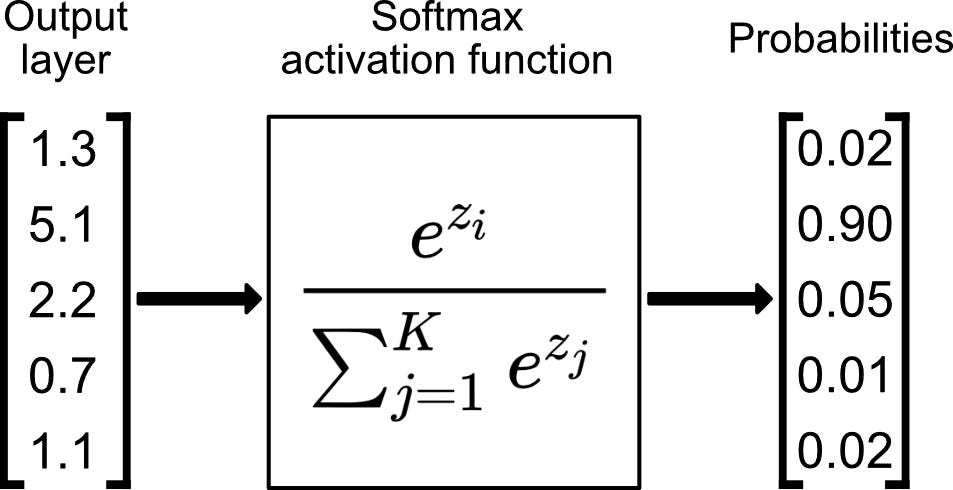
\includegraphics[width=0.6\linewidth]{images/softmaxworkingsimple.jpg}
\vspace{6pt}

To address this issue, alternative softmax implementations have been proposed, such as logsoftmax and Gumbel-Softmax, which aim to reduce the computational complexity while maintaining performance. In this article, I try to implement and understand the performance differences between various implementations.

\section{Methodology}


In this study, we employ the CIFAR-100 dataset, consisting of 100 classes of images, to compare the performance of different softmax variations in CNN models. First I developed a baseline CNN model with the standard softmax implementation. Then, created additional models using the same architecture but replacing the softmax layer with logsoftmax and Gumbel-Softmax, etc.

\textbf{Architecture of the model}


The CNN is architected on Resnet12 model. I tried creating my own CNN with several Convolution and activation layers, but accuracy was less compared when compared to already established layer architectures as that of Resnet12.

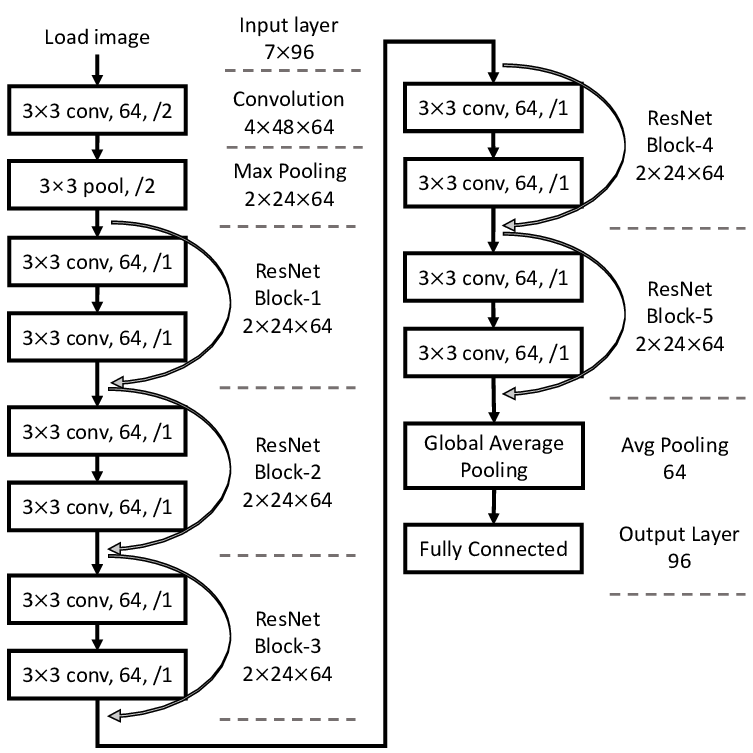
\includegraphics[scale=0.3]{images/The-structure-of-ResNet-12.png}

\subsection{Standard Softmax}

The standard softmax function is a commonly used activation function in neural networks for multiclass classification problems. Given an input vector, the softmax function transforms it into a vector of probabilities, where each element represents the probability of the input belonging to a particular class. The softmax function is defined as follows:

\[
\text{softmax}(x_i) = \frac{e^{x_i}}{\sum_{j=1}^{N}e^{x_j}}
\]

where \(x_i\) is the \(i\)-th element of the input vector, and \(N\) is the total number of classes.

The softmax function computes the exponentiated value of each element in the input vector and normalizes it by the sum of all exponentiated values. This normalization ensures that the output probabilities sum up to 1.


On adding the Softmax layer to the base model, the training results were as follows: \\

\begin{center}
\begin{tabular}{ |c|c|c|c| } 
 \hline
 Accuracy & Precision & Recall & F1 Score \\ 
 8.09\% & 0.0115 & 0.0817 & 0.02 \\
 \hline
\end{tabular}
\end{center}

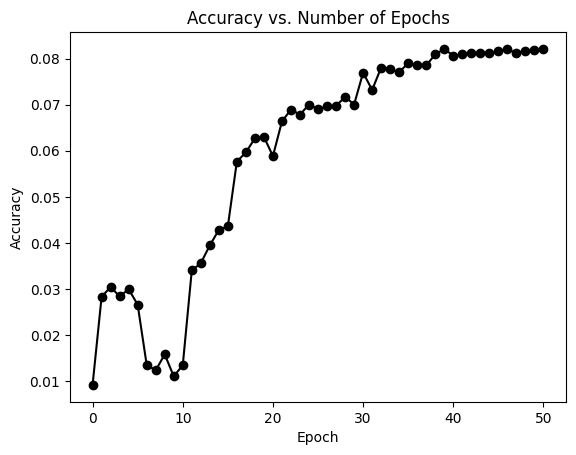
\includegraphics[width=0.5\linewidth]{images/Softmax/accvsloss.png}
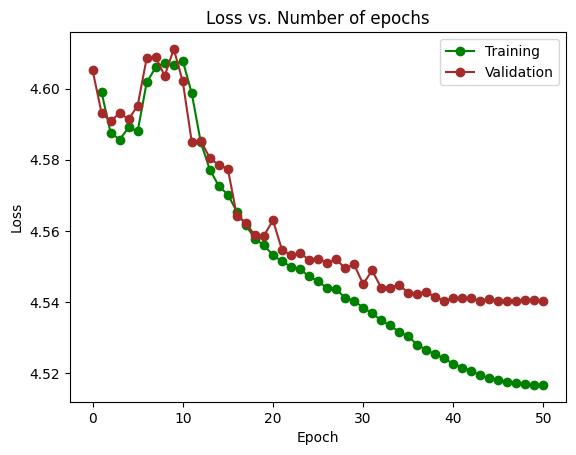
\includegraphics[width=0.5\linewidth]{images/Softmax/lossvsepochs.png}
\vspace{6pt}


\textbf{Confusion Matrix}

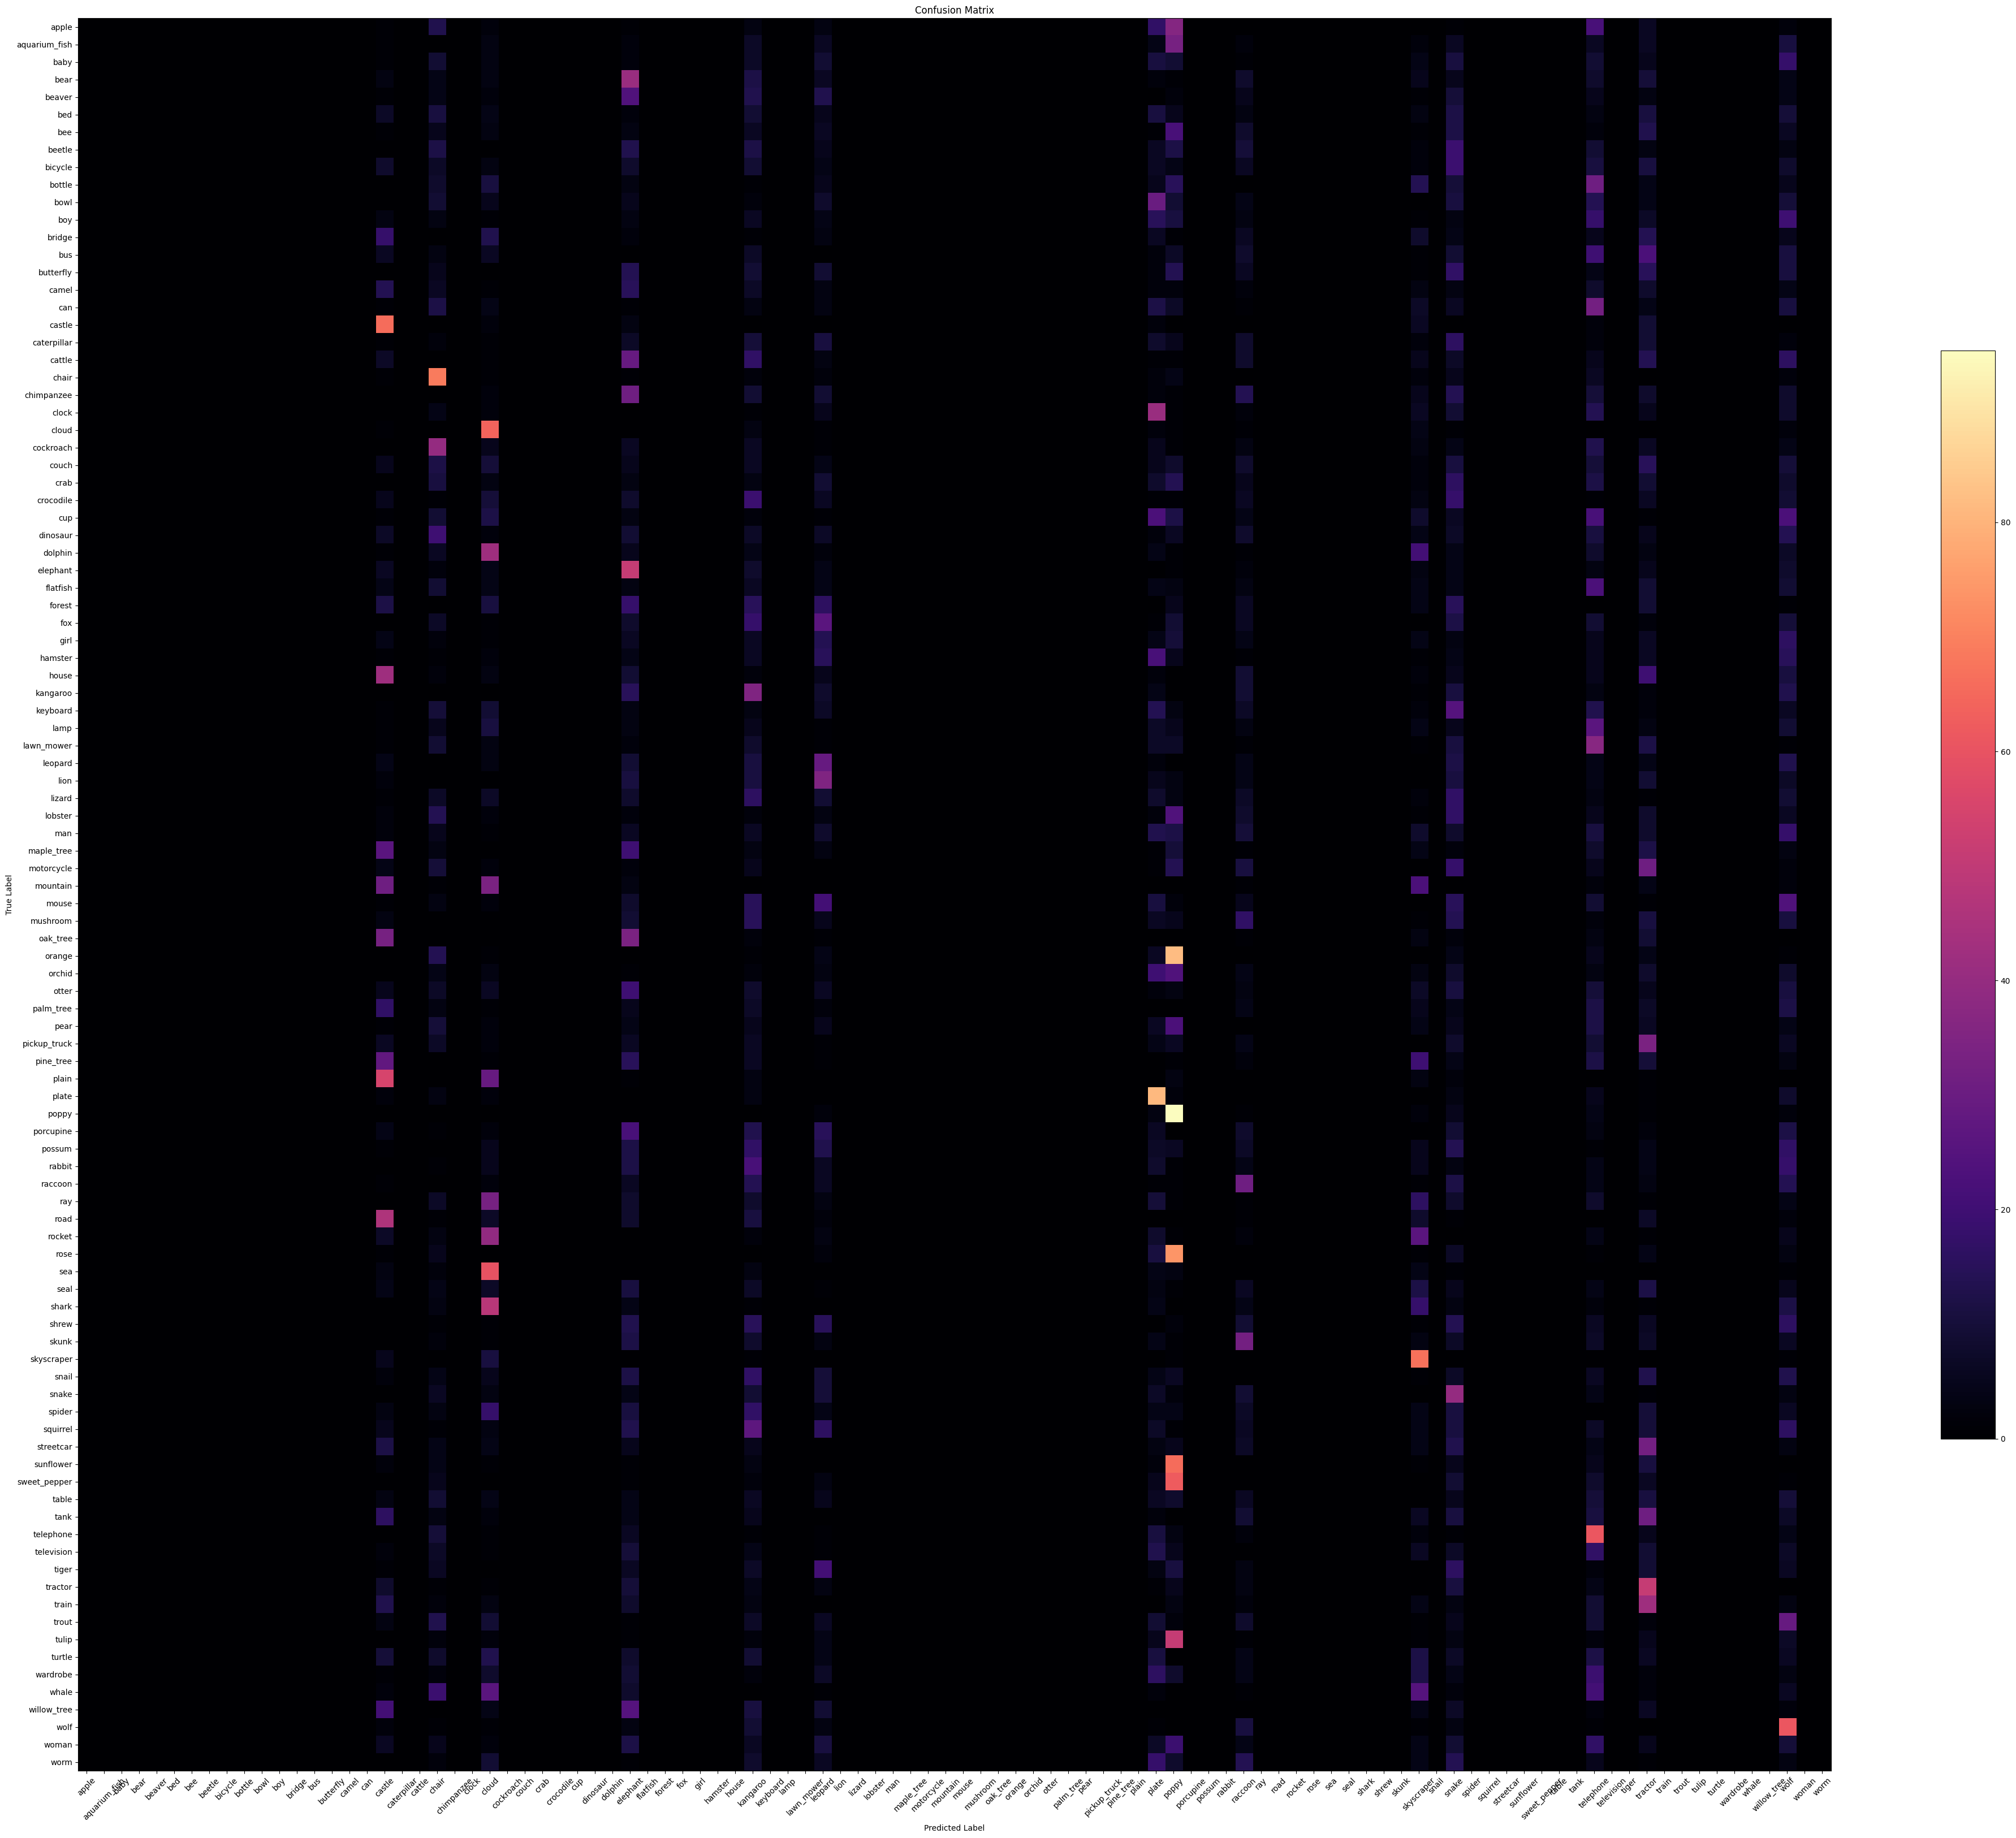
\includegraphics[width=0.9\linewidth]{images/Softmax/highres-softmax-resnet12.png}


\subsection{LogSoftmax}


The logsoftmax function is an alternative to the standard softmax function that can provide computational advantages. Instead of directly computing the softmax probabilities, the logsoftmax function calculates the logarithm of the softmax probabilities. The logsoftmax function is defined as follows:

\[
\text{LogSoftmax}(x_i) = \log\left(\frac{e^{x_i}}{\sum_{j=1}^N e^{x_j}}\right)
\]
can also be equalized to
\[
\text{logsoftmax}(x_i) = x_i - \log\left(\sum_{j=1}^{N}e^{x_j}\right)
\]

The logsoftmax function retains the relative order of the probabilities while reducing the computational complexity. It is often used in combination with the negative log-likelihood loss function, also known as cross-entropy loss, for training neural networks.

On implementing LogSoftmax instead of standard softmax, the accuracy improved drastically. This seems to be due to the fact that when using normal softmax, the vectors being exponentiated, increase the error by a lot; heavily hindering the performance of the model. But log softmax, simply converts vectors into probability, rather then exponential average. Not only does this reduce complexity but maintains the relative difference, which in this case seems to have helped.

\begin{center}
\begin{tabular}{ |c|c|c|c| } 
 \hline
 Accuracy & Precision & Recall & F1 Score \\ 
 60.16\% & 0.5922 & 0.5987 & 0.5931 \\
 \hline
\end{tabular}
\end{center}

        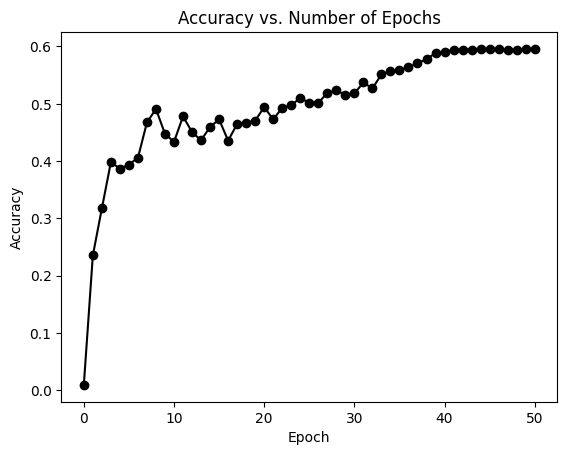
\includegraphics[width=0.5\linewidth]{images/LogSoftmax/logsoftmax-accepoch.png}
        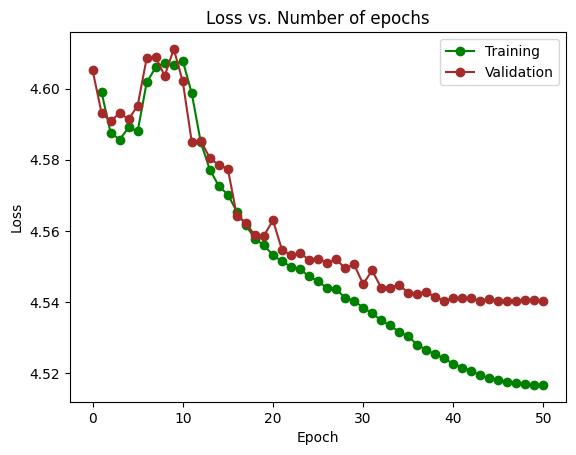
\includegraphics[width=0.5\linewidth]{images/LogSoftmax/logsoftmax-lossepoch.png}

\textbf{Confusion Matrix}

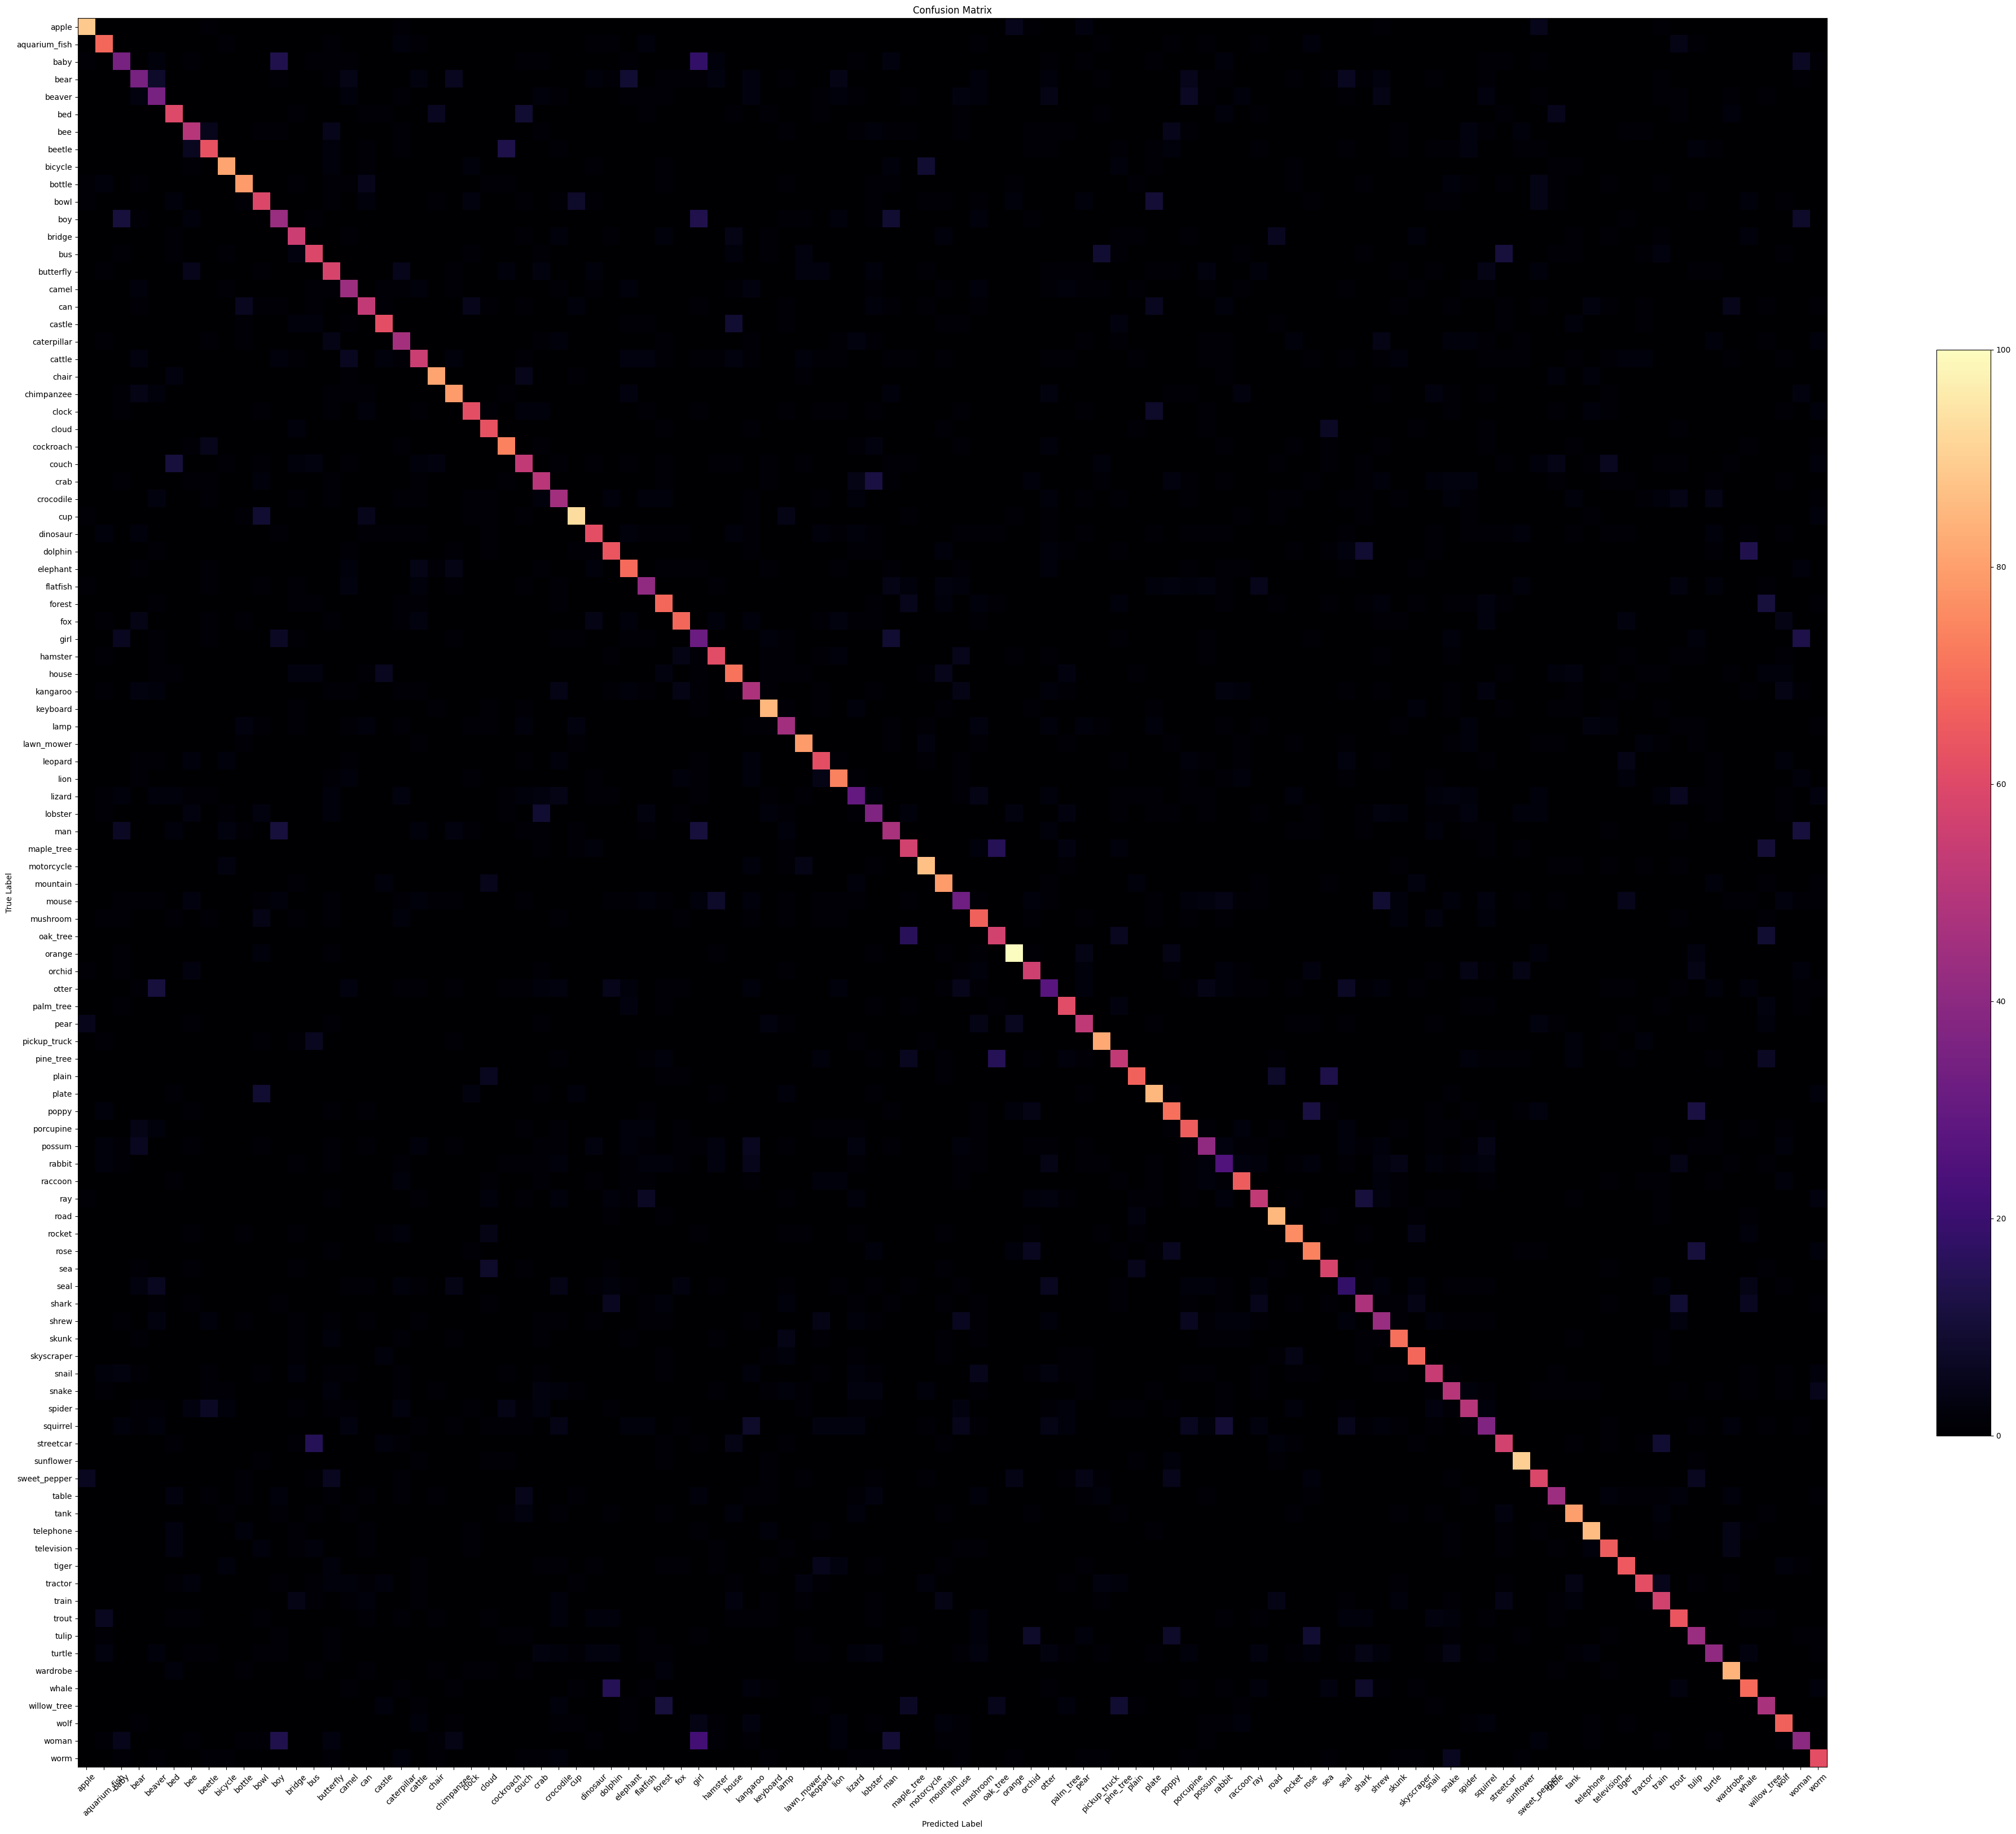
\includegraphics[width=0.9\linewidth]{images/LogSoftmax/highres-logsoftmax.png}
--

\subsection{Gumbel Softmax}

Gumbel-Softmax\cite{gumbel} is another alternative to the standard softmax function that introduces a stochastic component. It uses the Gumbel-Max trick to sample from the softmax distribution efficiently. The Gumbel-Softmax function is defined as follows:

\[
\text{Gumbel-Softmax}(x_i) = \frac{\exp((\log(p_i) + g_i)/\lambda)}{\sum_{j=1}^{N}\exp((\log(p_j) + g_j)/\lambda)}
\]

where \(p_i\) is the \(i\)-th element of the input vector, \(g_i\) is a sample from the Gumbel distribution, and \(\lambda\) is a temperature parameter that controls the smoothness of the distribution. The Gumbel-Softmax function approximates the softmax function while introducing randomness through the Gumbel noise.

This variation of softmax is just like standard softmax with a temperature term, "reducing" the vectors.

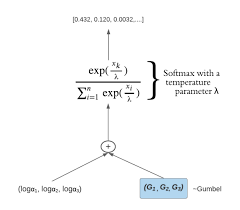
\includegraphics{images/lolgumbelsoftmax.png}

On training the model on this I could see an increase in the accuracy of the model on increasing the value of \(\lambda\).

\begin{center}
\begin{tabular}{ |c|c|c|c| } 
 \hline
 Accuracy & Precision & Recall & F1 Score \\ 
 11.83\% & 0.0244 & 0.1168 & 0.396 \\
 \hline
\end{tabular}
\end{center}

The above accuracy was with the value of \(\lambda\)= 3, on having value <=1 the accuracy didn't even reach 8\%. Overall the learning rate wrt the number of epochs didn't change much.


        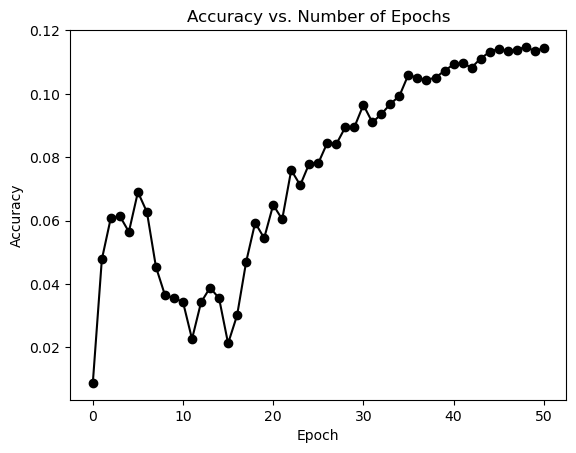
\includegraphics[width=0.5\linewidth]{images/GumbelSoftmax/gumbel-acc-epoch.png}
        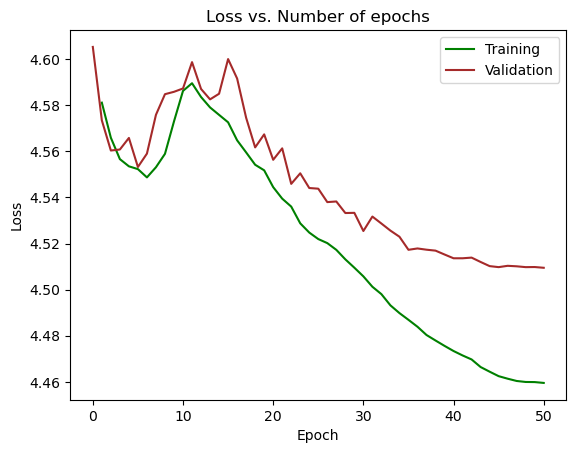
\includegraphics[width=0.5\linewidth]{images/GumbelSoftmax/gumbel-loss-epoch.png}

\textbf{Confusion Matrix}

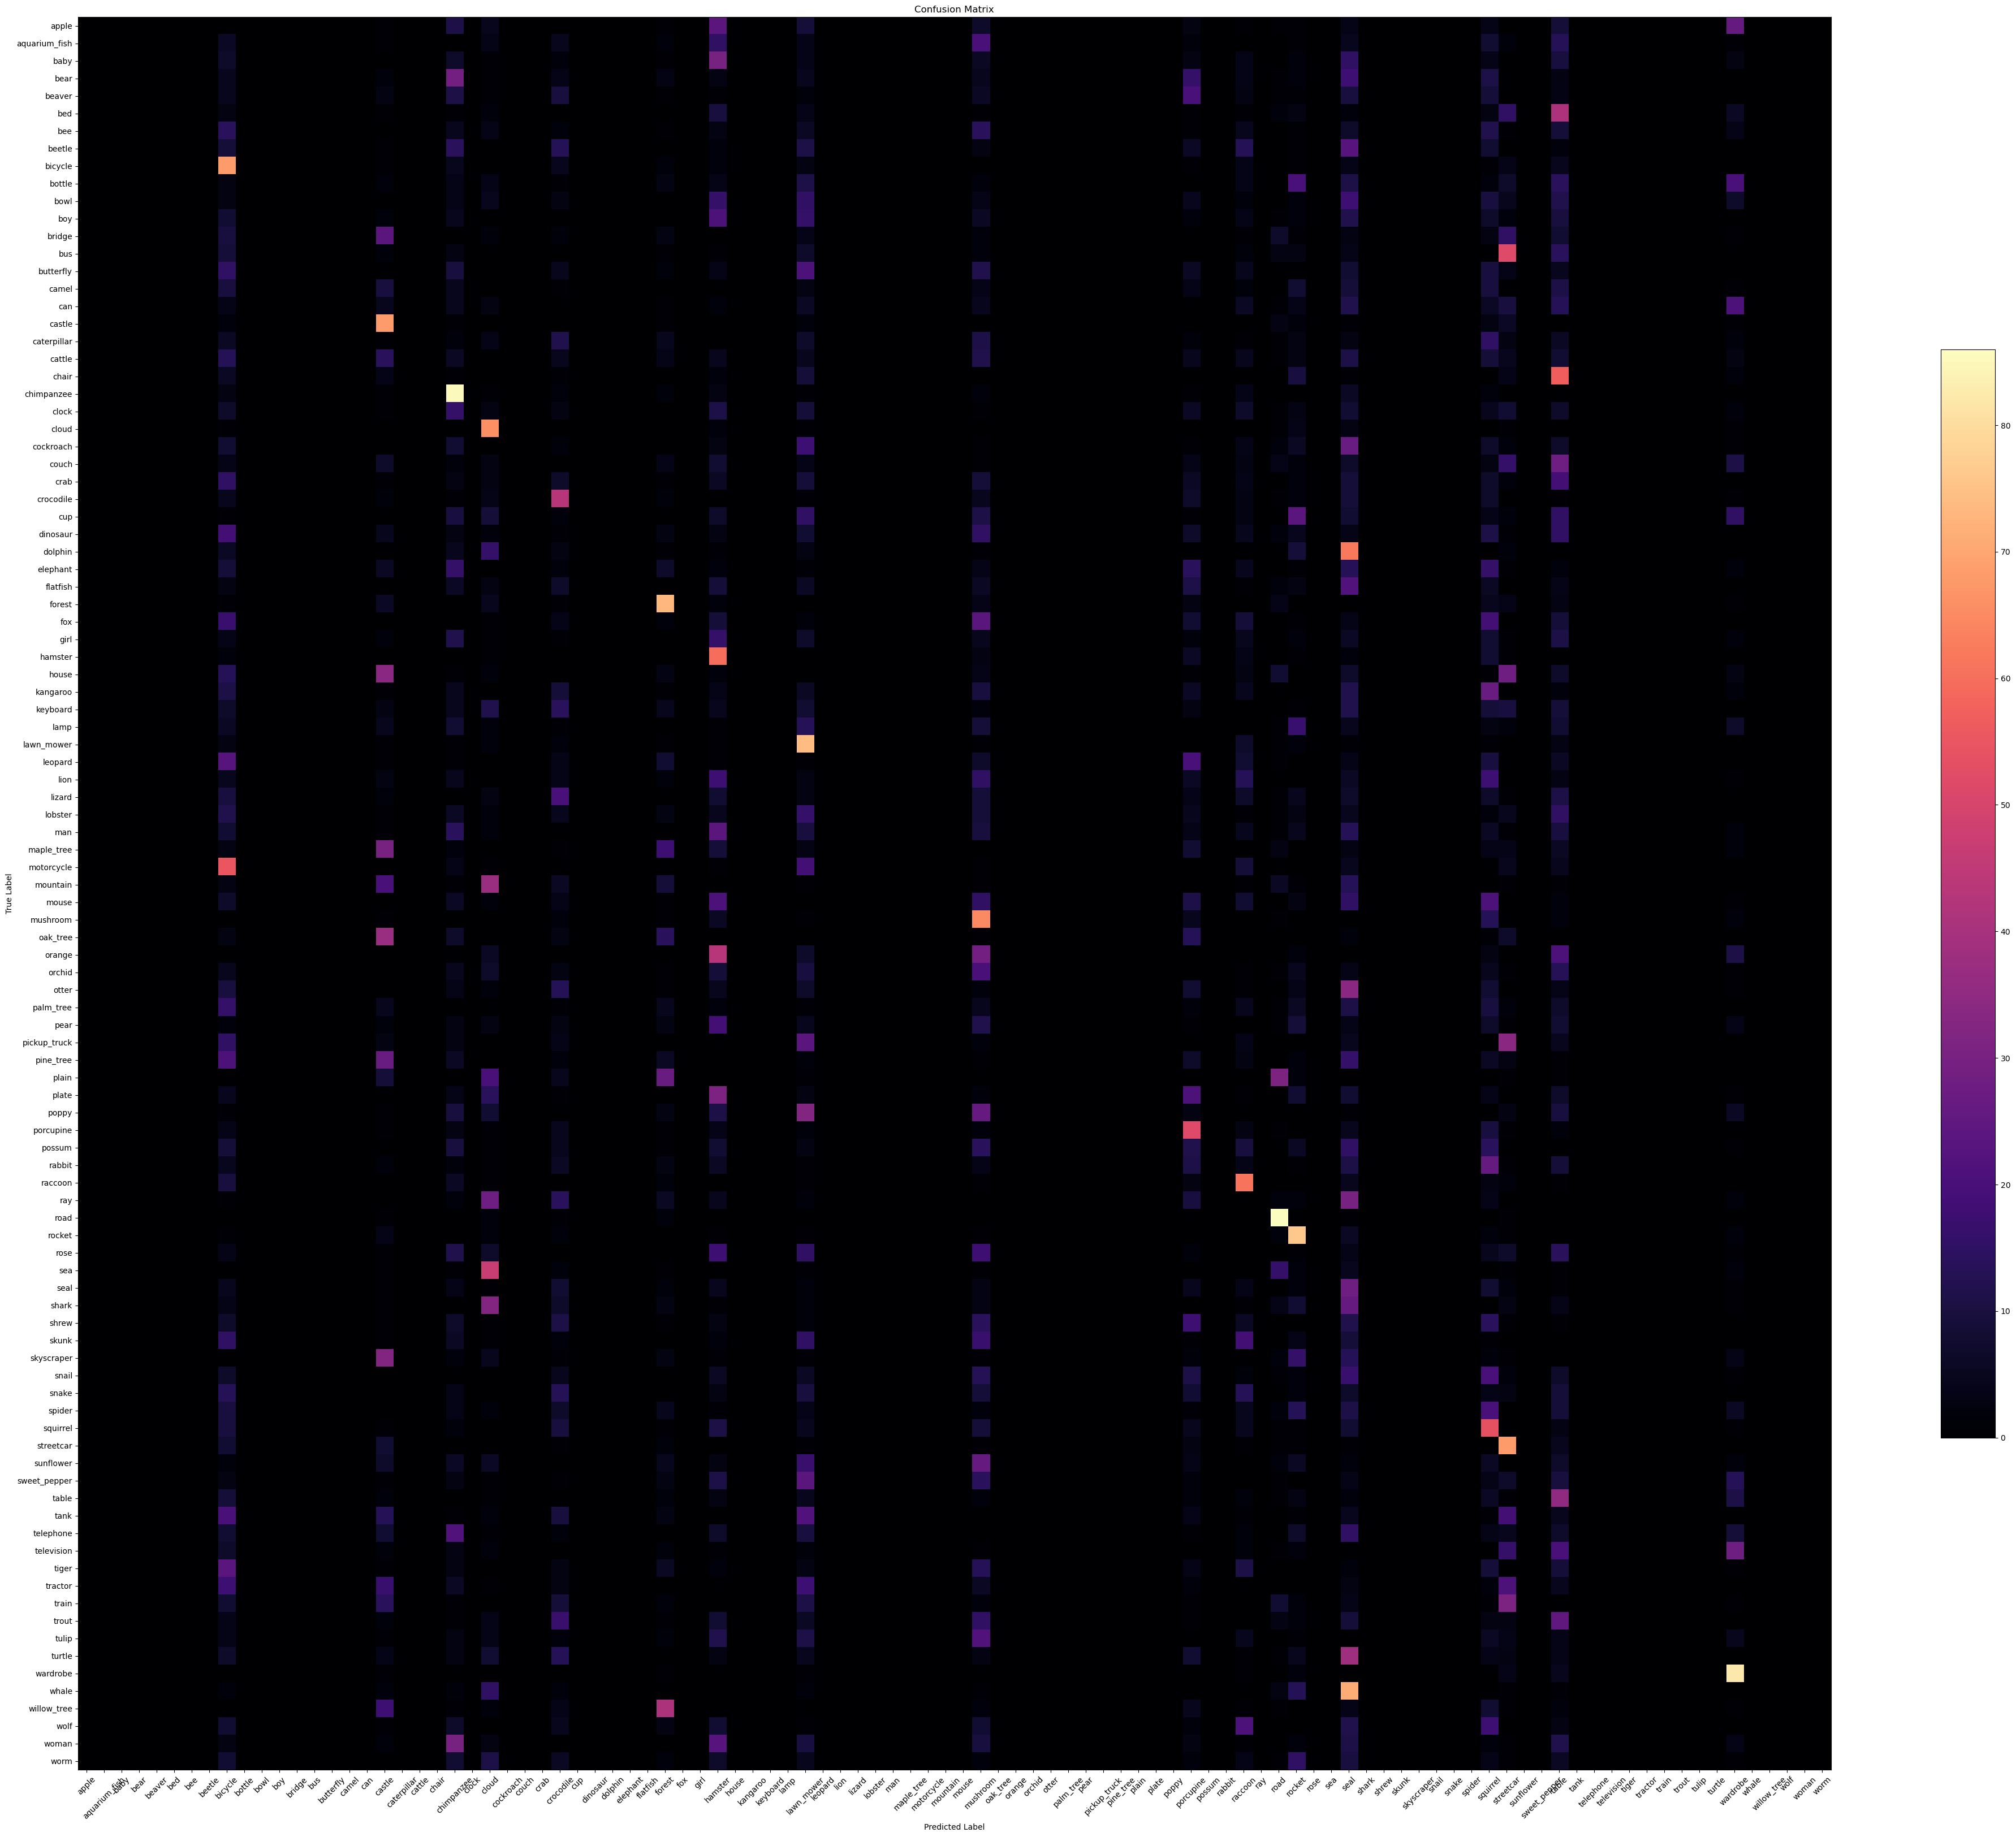
\includegraphics[width=0.9\linewidth]{images/GumbelSoftmax/gumbel-cm.png}

--
\vspace{6pt}
For \(\lambda\) = -1.5:

\begin{center}
\begin{tabular}{ |c|c|c|c| } 
 \hline
 Accuracy & Precision & Recall & F1 Score \\ 
 8.81\% & 0.0155 & 0.0888 & 0.0258 \\
 \hline
\end{tabular}
\end{center}

Gumbel like softmax gives poor performance. The scaling factor of lambda, does help as it reduces the exponents (explained later), but this approach does not scale well with classes.



\subsection{Log Gumbel Softmax}

The Log Gumbel-Softmax function is derived from the Gumbel-Softmax function by taking the logarithm of the probabilities. The Gumbel-Softmax function introduces stochasticity through Gumbel noise and approximates the softmax function. The Log Gumbel-Softmax function extends this by applying the logarithm.

Let's denote the input vector as \(x\) and the temperature parameter as \(\lambda\). The Log Gumbel-Softmax function is defined as follows:

\[
\text{LogGumbelSoftmax}(x_i) = \log\left(\frac{\exp((\log(p_i) + g_i)/\lambda)}{\sum_{j=1}^{N}\exp((\log(p_j) + g_j)/\lambda)}\right)
\]

where \(p_i\) is the \(i\)-th element of the input vector, \(g_i\) is a sample from the Gumbel distribution, and \(N\) is the total number of classes.

The Gumbel noise introduces randomness and allows for the relaxation of discrete distributions into continuous relaxations. The temperature parameter \(\lambda\) controls the smoothness of the distribution and the trade-off between exploration and exploitation.

\vspace{6pt}
For \(\lambda\) = 3:

\begin{center}
\begin{tabular}{ |c|c|c|c| } 
 \hline
 Accuracy & Precision & Recall & F1 Score \\ 
 61.04\% & 0.6033 & 0.6091 & 0.6035 \\
 \hline
\end{tabular}
\end{center}


        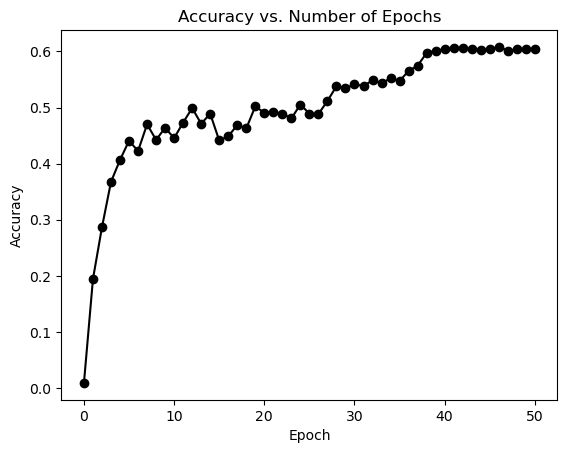
\includegraphics[width=0.5\linewidth]{images/LogGumbelSoftmax/log-gumbel-acc-epoch.png}
        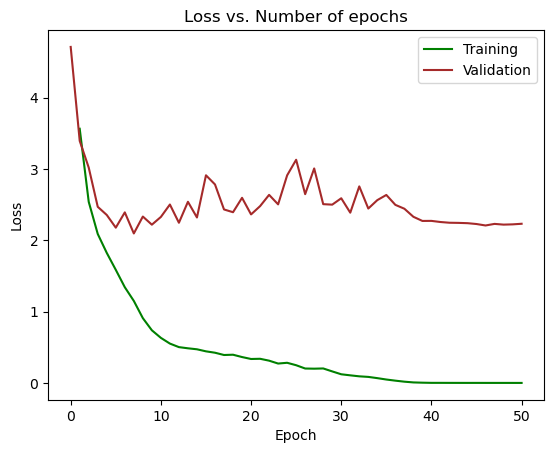
\includegraphics[width=0.5\linewidth]{images/LogGumbelSoftmax/log-gumbel-loss-epoch.png}

\textbf{Confusion Matrix}

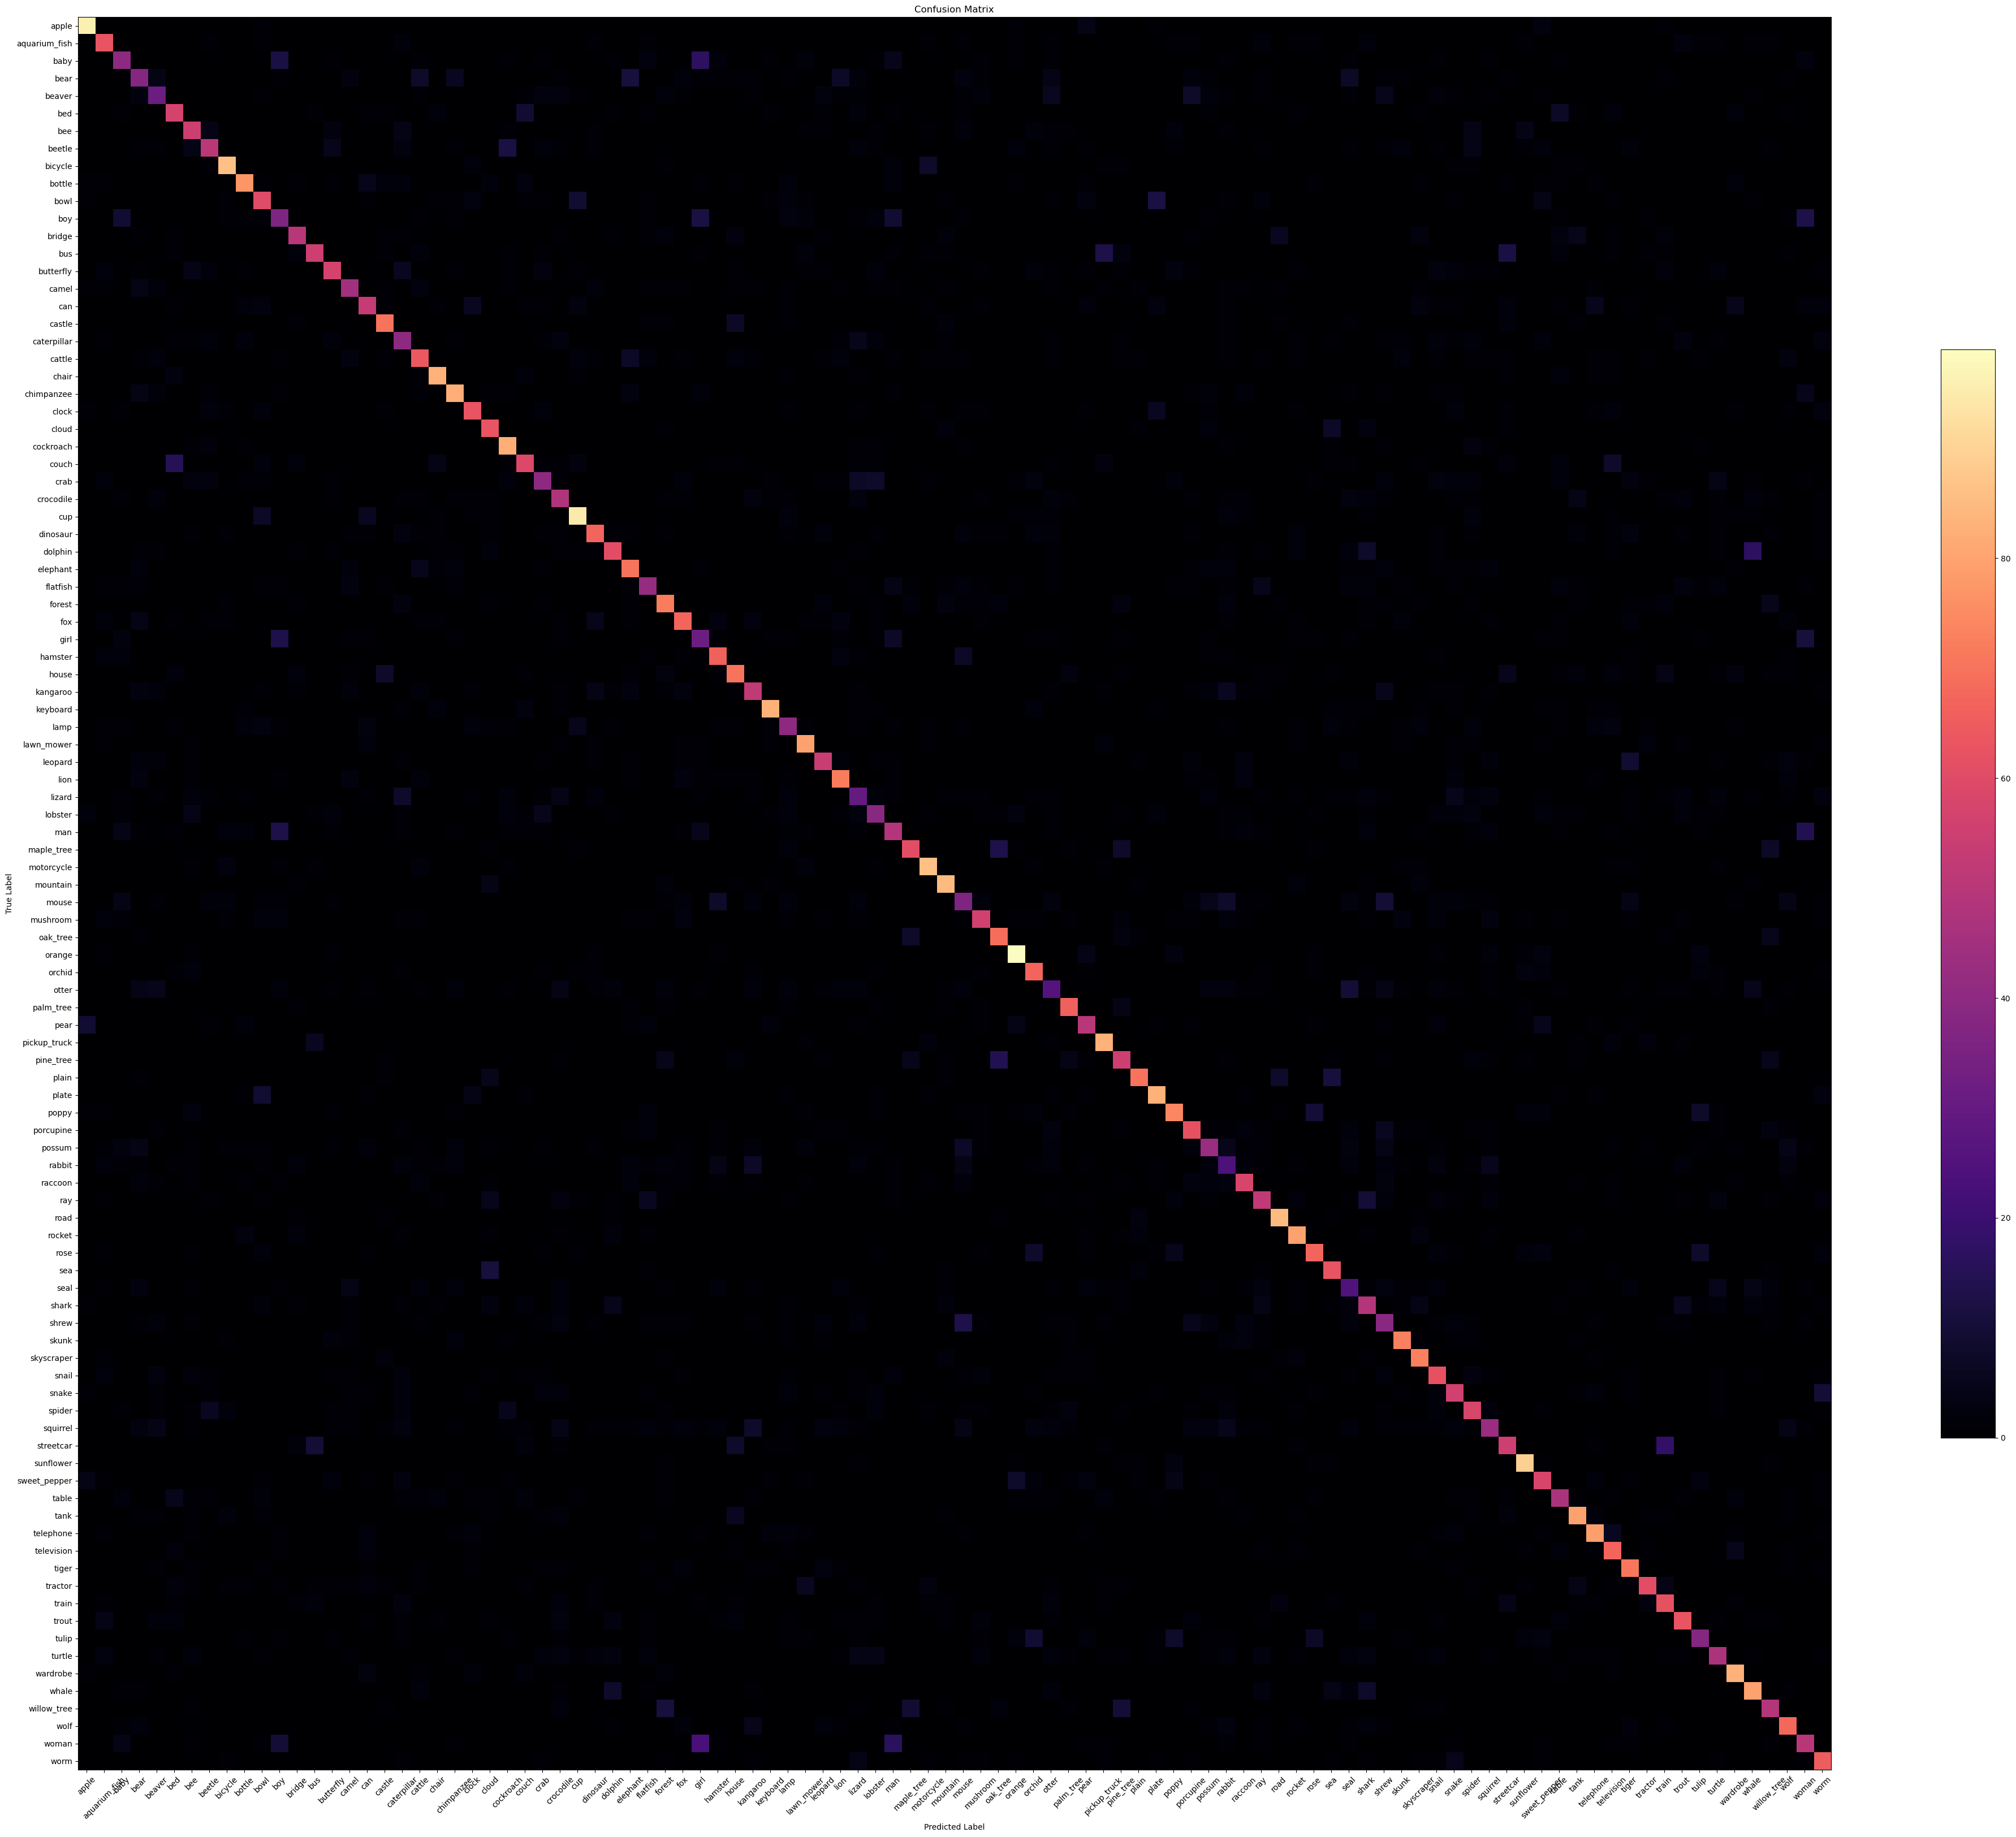
\includegraphics[width=0.9\linewidth]{images/LogGumbelSoftmax/cm-loggumbel.png}

--

\vspace{6pt}
For \(\lambda\) = -1.5:

\begin{center}
\begin{tabular}{ |c|c|c|c| } 
 \hline
 Accuracy & Precision & Recall & F1 Score \\ 
 59.44\% & 0.5846 & 0.5899 & 0.5850 \\
 \hline
\end{tabular}
\end{center}

--



\subsection{Other tries}

What if instead of have \(e^z\) we have \(2^z\) in the softmax function. This does not change a lot in terms of mathematical operations, but does help in computational scaling. As by the use of bitwise operator computers can quickly calculate \(2^z\). This does not seem to do anything, as it is the same computation. Although on using low level operations, by using bitwise operations, such \(2^z_i\) operations can be optimized.

I tried various other variations of softmax-like operations: 

- \(e^P[Z<z_i]\)

- \(e^sin(z_i\)

- Sparsemax\cite{sparsemax}

None of these gave decent accuracies. All were around that of Softmax, with similar functioning.



\section{Hypothesis}

\subsection{Reason for low performance of Softmax, when compared to others}

To compare the accuracy of softmax and log softmax, let's consider a 1D array as an example: [13, 8, 2]. We will calculate the probabilities using both softmax and log softmax and analyze the differences.

\textbf{Softmax}

The softmax function transforms the input vector into a probability distribution. Let's calculate the softmax probabilities for the given array.

\[
\text{Softmax}([13, 8, 2]) = \left[\frac{e^{13}}{e^{13}+e^8+e^2}, \frac{e^8}{e^{13}+e^8+e^2}, \frac{e^2}{e^{13}+e^8+e^2}\right]
\]

Calculating the exponential values:

\[
\text{Softmax}([13, 8, 2]) = \left[\frac{442413.39}{442413.39+2980.96+7.39}, \frac{2980.96}{442413.39+2980.96+7.39}, \frac{7.39}{442413.39+2980.96+7.39}\right]
\]

Normalizing the values:

\[
\text{Softmax}([13, 8, 2]) \approx [0.999, 0.001, 0]
\]

The softmax probabilities indicate that the first element has a high probability (approximately 99.9%) of belonging to the class, while the second element has a very low probability (approximately 0.1%), and the third element has an almost negligible probability.

\textbf{Log Softmax}

The log softmax function calculates the logarithm of the softmax probabilities. Let's calculate the log softmax probabilities for the same array.

\[
\text{Log Softmax}([13, 8, 2]) = \left[13 - \log(e^{13}+e^8+e^2), 8 - \log(e^{13}+e^8+e^2), 2 - \log(e^{13}+e^8+e^2)\right]
\]

Calculating the exponential values:

\[
\text{Log Softmax}([13, 8, 2]) = \left[13 - \log(442413.39+2980.96+7.39), 8 - \log(442413.39+2980.96+7.39), 2 - \log(442413.39+2980.96+7.39)\right]
\]

Normalizing the values:

\[
\text{Log Softmax}([13, 8, 2]) \approx [13 - 13.1, 8 - 13.1, 2 - 13.1] \approx [-0.1, -5.1, -11.1]
\]

The log softmax probabilities indicate that the first element has a relatively high value (-0.1), the second element has a lower value (-5.1), and the third element has the lowest value (-11.1).

\textbf{Reasoning}

The difference in accuracy between softmax and log softmax arises from the nature of the functions and the properties they preserve.

Softmax calculates the exponential values of the input vector, which can lead to significant differences in magnitudes. In our example, the element with the highest value (13) has a much larger exponential value compared to the other elements. This exponential amplification causes the softmax probabilities to be heavily skewed towards the highest value, resulting in a very high probability for the first element and extremely low probabilities for the other elements.

On the other hand, log softmax calculates the logarithm of the softmax probabilities. Taking the logarithm dampens the differences in magnitudes and compresses the range of values. In our example, the log softmax probabilities are relatively close to each other (-0.1, -5.1, -11.1), indicating a more balanced distribution of probabilities among the elements.

The log softmax function is therefore preffered over softmax when dealing with models that have a large output space like image classification of larger datasets. By taking the logarithm, log softmax reduces the chances of numerical overflow or underflow that can occur with softmax, especially when dealing with large or small exponentiated values.

In terms of accuracy, log softmax is much more balanced and probabilities are more useful when compared to softmax, especially in scenarios where there are significant differences in the magnitudes of the input vector elements.

\subsection{Using 20 Super Classes}

When I trained the model on just the 20 super classes, the accuracy with activation layer being Softmax for 50 epochs was ~ 45\% , which decreases drastically on increasing it to 100 classes. Further showing that the complexity increases drastically with increasing the number of classes.

\vspace{6pt}
\vspace{6pt}

Other references
\cite{cifar100}
\cite{fast-softmax-sampling} \cite{maddison2017concrete} \cite{alitabakds_my-first-project_2023}


\bibliography{test}



\end{document}
